\documentclass[aspectratio=169,11pt]{beamer}
\usetheme{metropolis}
\metroset{block=fill, numbering=fraction, progressbar=frametitle}

% - Encoding & Vietnamese -
\usepackage[utf8]{inputenc}
\usepackage[T5]{fontenc}
\usepackage[vietnamese]{babel}

% - Packages -
\usepackage{booktabs}
\usepackage{amsmath, amssymb}
\usepackage{graphicx}
\usepackage{tikz}
\usetikzlibrary{shapes.geometric, arrows.meta, positioning}

% - Mau accent -
\definecolor{accent}{HTML}{2C6E72}
\setbeamercolor{frametitle}{bg=accent}
\setbeamercolor{progress bar}{fg=accent}

% - Custom commands -
\newcommand{\CR}{\ensuremath{\mathrm{CR}}}
\newcommand{\Cu}{\ensuremath{C_u}}
\newcommand{\Co}{\ensuremath{C_o}}

\graphicspath{{figures/}}
\setlength{\emergencystretch}{3em}  % tranh tran dong nho voi tu tieng Anh khong ngat duoc

% - Title -
\title{Hệ hỗ trợ quyết định đặt hàng}
\subtitle{Dự báo chuỗi thời gian đa phân vị \& tối ưu hóa tồn kho}
\author{Nguyễn Trường Giang \\ \small MSSV 20227044 --- GVHD: TS. Nguyễn Hữu Du}
\institute{Đại học Bách khoa Hà Nội --- Khoa Toán -- Tin\\ \textit{Đồ án 1}}
\date{Tháng 6, 2025}

\begin{document}

\maketitle

\begin{frame}{Nội dung}
  \setbeamertemplate{section in toc}[sections numbered]
  \tableofcontents[hideallsubsections]
\end{frame}

% ============================================================
\section{Bài toán}
% ============================================================

\begin{frame}{``Tháng này nên đặt bao nhiêu hàng?''}
  Một câu hỏi đơn giản, hai rủi ro đối lập:
  \begin{itemize}
    \item \textbf{Đặt ít} $\rightarrow$ hết hàng $\rightarrow$ mất doanh thu, mất khách.
    \item \textbf{Đặt nhiều} $\rightarrow$ tồn ế $\rightarrow$ ứ đọng vốn, hao hụt.
  \end{itemize}
  \vfill
  \begin{alertblock}{Khó khăn cốt lõi}
    Nhu cầu tương lai \textbf{không chắc chắn}. Dự báo điểm (một con số) bỏ qua
    thông tin quan trọng nhất: \textbf{phân phối xác suất} của nhu cầu --- thứ
    quyết định mức tồn kho tối ưu về kinh tế.
  \end{alertblock}
\end{frame}

\begin{frame}{Ai dùng \& cần quyết định gì?}
  \begin{columns}[T]
    \begin{column}{0.5\textwidth}
      \textbf{Người sử dụng}
      \begin{itemize}
        \item Quản lý kinh doanh --- cần con số khuyến nghị \emph{dễ hiểu}.
        \item Phân tích cung ứng --- cần \emph{chi tiết} dự báo \& độ tin cậy.
      \end{itemize}
    \end{column}
    \begin{column}{0.5\textwidth}
      \textbf{Quyết định cần hỗ trợ}
      \begin{itemize}
        \item Lượng hàng đặt thêm cho tháng tới \,(\textbf{Newsvendor}).
        \item Cỡ lô \& điểm đặt lại dài hạn \,(\textbf{EOQ}).
      \end{itemize}
    \end{column}
  \end{columns}
  \vfill
  \begin{block}{Ý tưởng cốt lõi}
    Dự báo \textbf{cả phân phối} nhu cầu (đa phân vị), rồi để \textbf{cấu trúc chi
    phí} của doanh nghiệp tự chọn mức chuẩn bị tối ưu.
  \end{block}
\end{frame}

\begin{frame}{Kiến trúc hệ thống}
  \centering
  \resizebox{\textwidth}{!}{%
  \begin{tikzpicture}[
    node distance=0.6cm and 0.7cm,
    box/.style={draw, rounded corners=3pt, fill=accent!12, text width=2.4cm,
                align=center, minimum height=1.2cm, font=\footnotesize},
    arr/.style={-{Stealth[length=2mm]}, thick}]
    \node[box] (data) {Dữ liệu tháng\\(120 obs)};
    \node[box, right=of data, fill=accent!22] (model) {RevIN +\\N-BEATS};
    \node[box, right=of model] (dist) {Phân phối\\P5--P95};
    \node[box, right=of dist, fill=orange!18] (nv) {Newsvendor\\/ EOQ};
    \node[box, right=of nv, fill=orange!30] (dec) {Quyết định\\đặt hàng};
    \draw[arr] (data) -- (model);
    \draw[arr] (model) -- (dist);
    \draw[arr] (dist) -- (nv);
    \draw[arr] (nv) -- (dec);
  \end{tikzpicture}}
  \vfill
  \begin{itemize}
    \item \textbf{Dự báo} cung cấp toàn bộ phân phối nhu cầu, không chỉ một con số.
    \item \textbf{Tối ưu tồn kho} biến phân phối đó thành khuyến nghị có ý nghĩa kinh tế.
  \end{itemize}
\end{frame}

% ============================================================
\section{Dữ liệu \& Phân tích khám phá}
% ============================================================

\begin{frame}{Dữ liệu}
  \begin{columns}[T]
    \begin{column}{0.42\textwidth}
      \begin{itemize}
        \item \textbf{120 tháng} (2015--2024).
        \item Mục tiêu: \texttt{Quantity}.
        \item 10 biến vĩ mô ngoại sinh.
        \item Chia theo thời gian \textbf{7:1:2}\\(train 84 / val 12 / test 24).
      \end{itemize}
      \vspace{0.3cm}
      {\footnotesize Tập test 24 tháng (2 năm) để đánh giá ổn định, đáng tin hơn.}
    \end{column}
    \begin{column}{0.58\textwidth}
      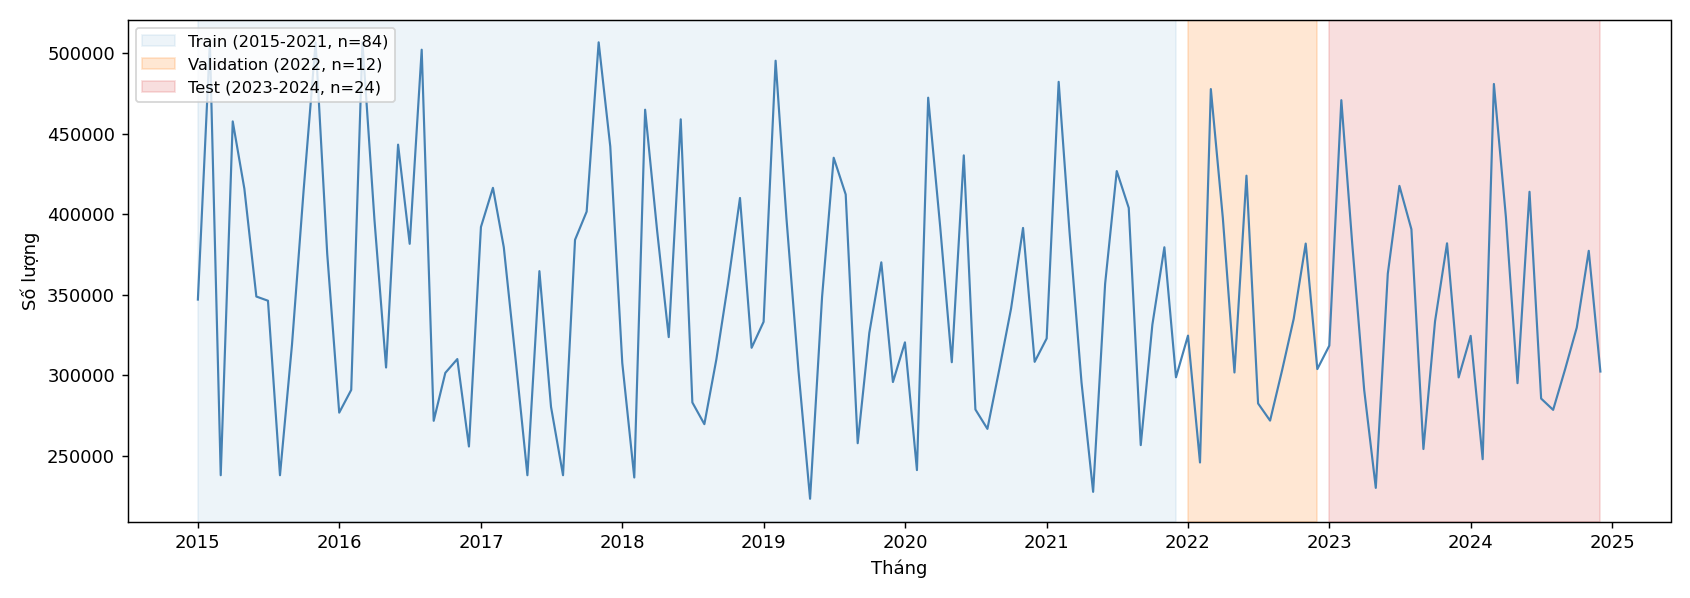
\includegraphics[width=\linewidth]{fig1_series_split}
    \end{column}
  \end{columns}
\end{frame}

\begin{frame}{Hai phát hiện EDA định hình phương pháp}
  \begin{columns}[T]
    \begin{column}{0.5\textwidth}
      \begin{itemize}
        \item \textbf{Distribution shift mạnh}: PromotionAmount tăng $\sim$90 lần
              trong 10 năm.\\ $\Rightarrow$ dùng \textbf{RevIN} (chuẩn hóa từng cửa sổ).
        \item \textbf{Mùa vụ yếu}, không cấu trúc AR/MA rõ.\\ $\Rightarrow$ dùng
              \textbf{N-BEATS} (MLP phi tuyến), không dùng ARIMA.
      \end{itemize}
    \end{column}
    \begin{column}{0.5\textwidth}
      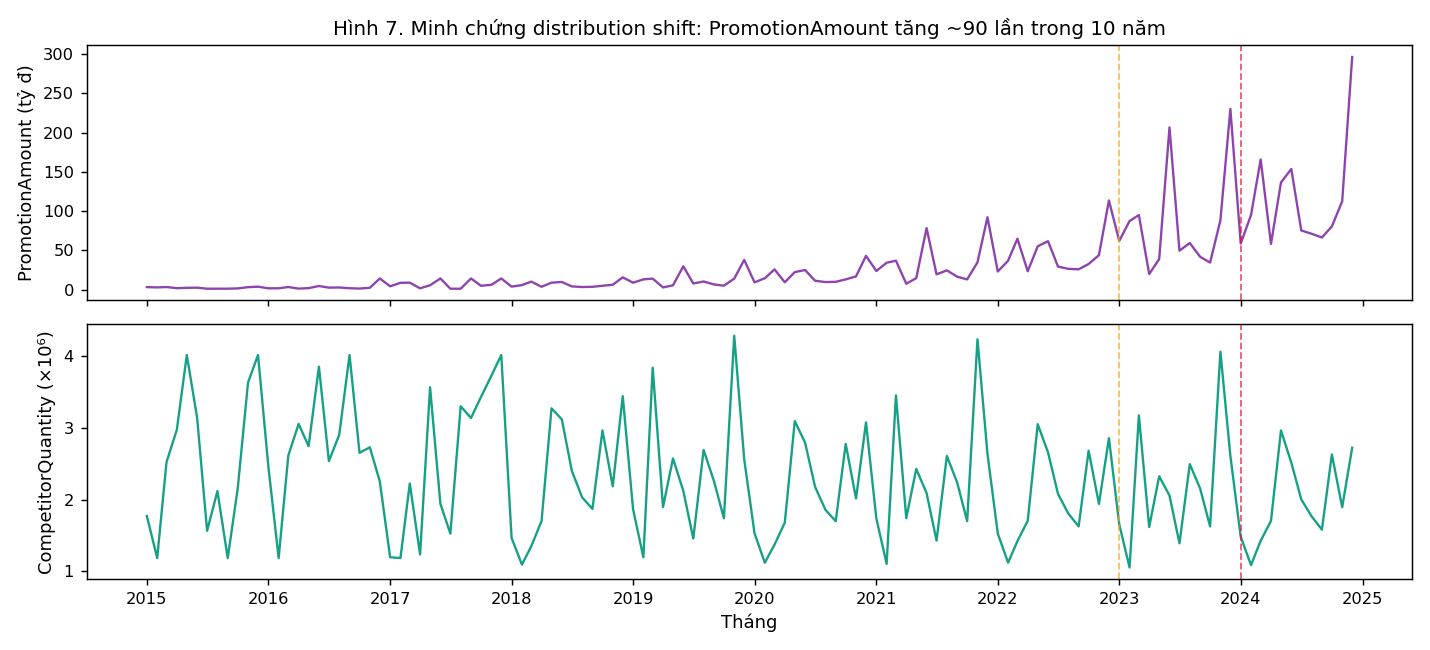
\includegraphics[width=\linewidth]{fig7_exog_trend}
    \end{column}
  \end{columns}
\end{frame}

% ============================================================
\section{Phương pháp}
% ============================================================

\begin{frame}{Lõi dự báo: RevIN + N-BEATS}
  \begin{columns}[T]
    \begin{column}{0.5\textwidth}
      \begin{block}{RevIN}
        \begin{itemize}\small
          \item Chuẩn hóa mean/std \emph{từng cửa sổ} đầu vào, đảo ngược ở đầu ra.
          \item Bất biến với mức nền thay đổi $\rightarrow$ chống distribution shift.
        \end{itemize}
      \end{block}
    \end{column}
    \begin{column}{0.5\textwidth}
      \begin{block}{N-BEATS}
        \begin{itemize}\small
          \item Chồng nhiều block MLP theo \emph{doubly-residual}: trừ backcast, cộng dồn forecast.
          \item Không hồi quy, học mẫu phi tuyến hiệu quả.
        \end{itemize}
      \end{block}
    \end{column}
  \end{columns}
  \vfill
  \centering\footnotesize
  Siêu tham số tối ưu bằng \textbf{Optuna} (100 trial): lookback 24, hidden 384,
  2 stack $\times$ 3 block, 3 lớp.
\end{frame}

\begin{frame}{Dự báo đa phân vị}
  \begin{itemize}
    \item Dự báo đồng thời \textbf{7 phân vị} P5, P10, P25, P50, P75, P90, P95
          $\rightarrow$ ước lượng cả phân phối nhu cầu.
    \item Huấn luyện bằng \textbf{pinball loss} --- chuẩn lý thuyết cho hồi quy phân vị.
    \item \textbf{RevIN}: chống distribution shift bằng chuẩn hóa theo từng cửa sổ.
  \end{itemize}
  \vfill
  \begin{block}{Đầu ra đơn điệu (không quantile crossing)}
    Tham số hóa \emph{base + cộng dồn softplus} đảm bảo
    $P5 \le P10 \le \cdots \le P95$ --- dùng chung cho mọi kiến trúc so sánh.
  \end{block}
\end{frame}

\begin{frame}{So sánh công bằng: mỗi mô hình tinh chỉnh Optuna riêng}
  \textbf{Mỗi mô hình} được Optuna tinh chỉnh riêng (100 trial); DLinear/TSMixer \emph{đa biến} (+6 ngoại sinh):
  \vspace{0.15cm}
  \begin{columns}[c]
    \begin{column}{0.5\textwidth}
      \scriptsize
      \begin{tabular}{lrr}
        \toprule
        Mô hình & MAE & Pinball \\
        \midrule
        Naive             & 80.045 & -- \\
        MLP               & 7.188 & 2.234 \\
        NHITS             & 6.937 & 1.977 \\
        TSMixer \tiny(đa biến) & 5.648 & 1.615 \\
        DLinear \tiny(đa biến) & 4.854 & 1.498 \\
        \textbf{N-BEATS}  & \textbf{3.894} & \textbf{1.145} \\
        \bottomrule
      \end{tabular}
      \vspace{0.2cm}
      \par{\scriptsize (test 24 tháng, 3 hạt giống)}
    \end{column}
    \begin{column}{0.5\textwidth}
      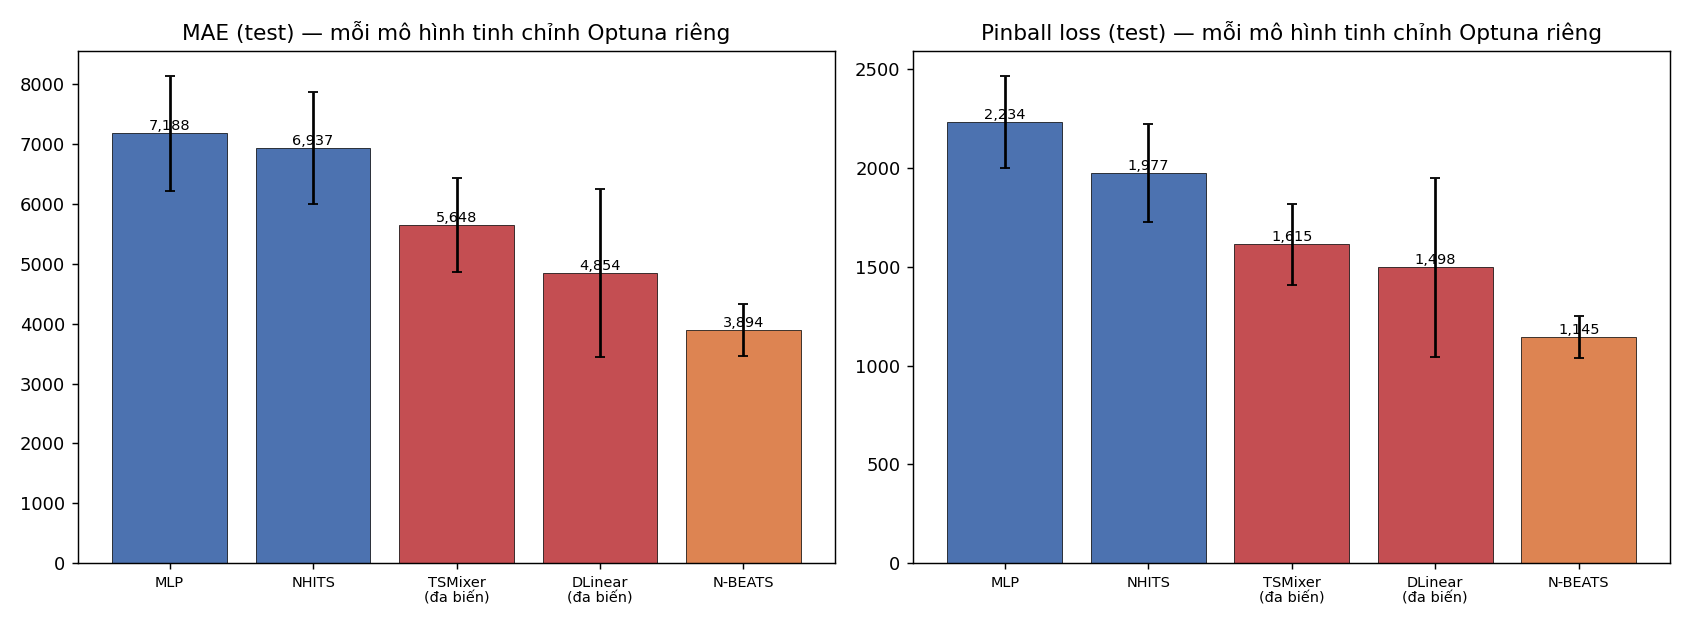
\includegraphics[width=\linewidth]{tune_all}
    \end{column}
  \end{columns}
  \vspace{0.1cm}
  {\small Khi tinh chỉnh công bằng, \textbf{N-BEATS tốt nhất rõ rệt} (mọi chỉ số).
  DLinear đa biến hạng nhì mà chỉ \textbf{2,4k tham số}.}
\end{frame}

% ============================================================
\section{Kết quả}
% ============================================================

\begin{frame}{Kết quả dự báo (tập test 24 tháng)}
  \begin{columns}[T]
    \begin{column}{0.36\textwidth}
      \begin{block}{N-BEATS tinh chỉnh}
        \begin{itemize}
          \item MAE = \textbf{4.074}
          \item MAPE = \textbf{1,15\%}
          \item RMSE = 5.090
        \end{itemize}
      \end{block}
      Vượt trội gần \textbf{20 lần} so với Naive (MAE 80.045).
    \end{column}
    \begin{column}{0.64\textwidth}
      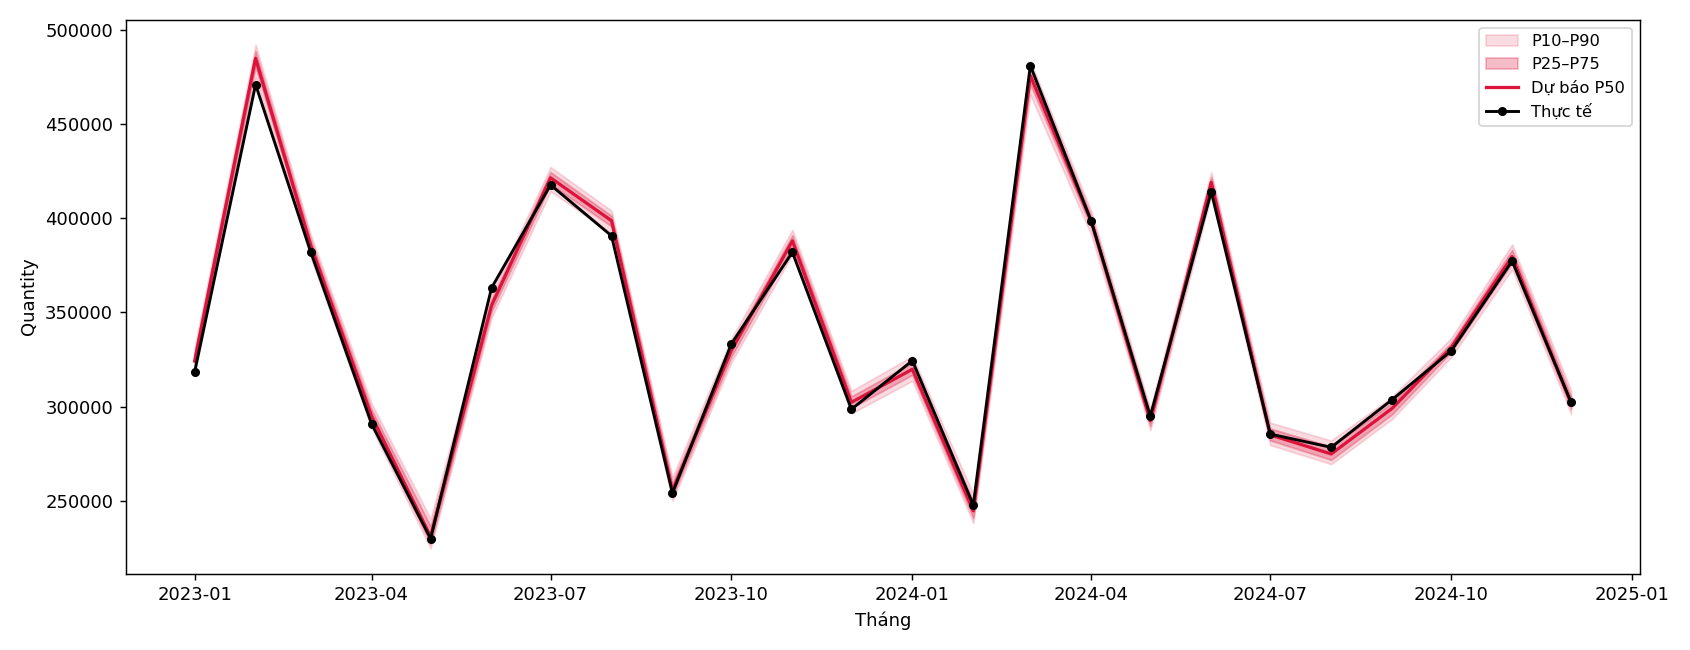
\includegraphics[width=\linewidth]{res1_test_forecast}
    \end{column}
  \end{columns}
\end{frame}

\begin{frame}{Dự báo phân vị 12 tháng tới (2025)}
  \begin{columns}[T]
    \begin{column}{0.62\textwidth}
      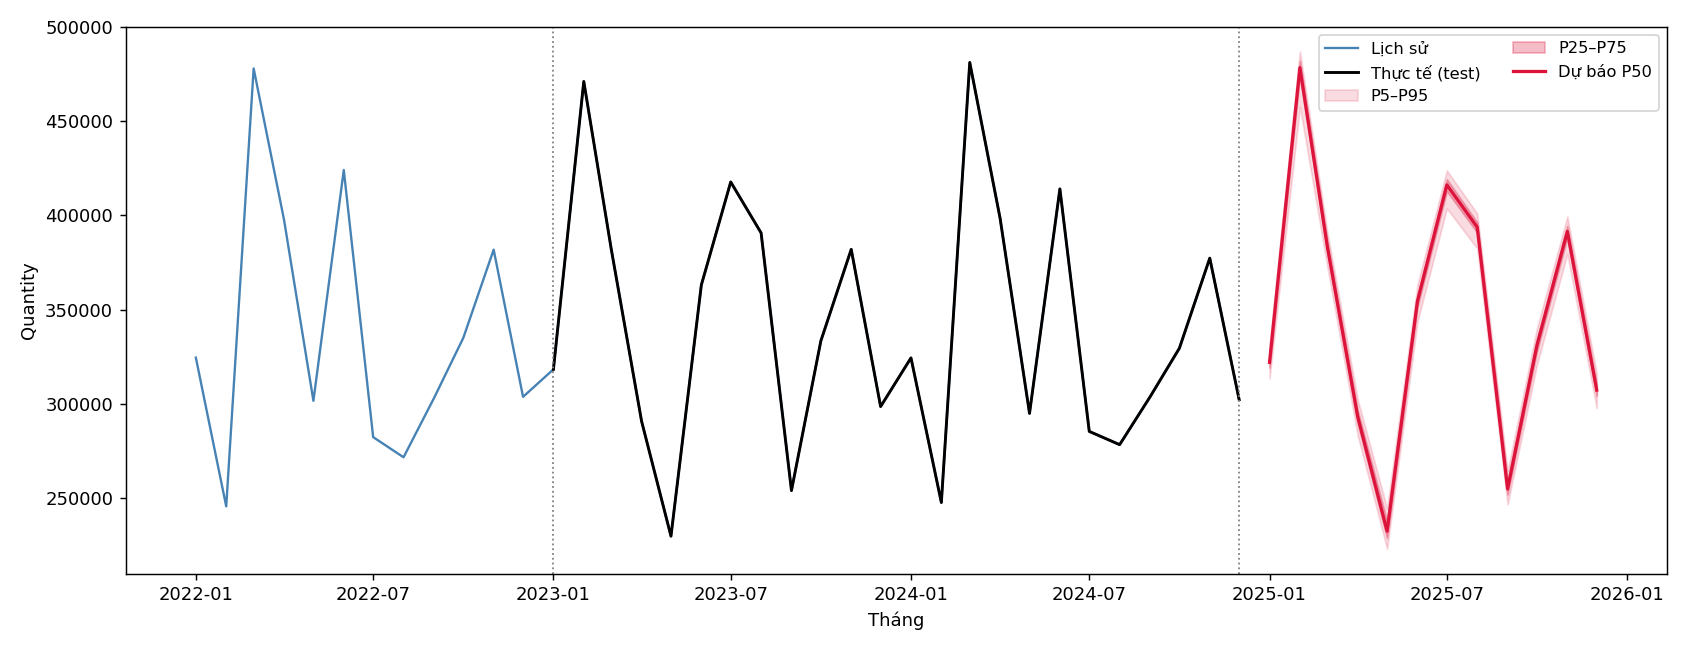
\includegraphics[width=\linewidth]{res2_fanchart}
    \end{column}
    \begin{column}{0.38\textwidth}
      \begin{itemize}
        \item Fan chart cho cả năm 2025: trung vị P50 + dải P5--P95.
        \item Khoảng \textbf{hẹp ở gần hạn} (tự tin cao), rộng dần khi xa.
        \item Đây là đầu ra trực tiếp đưa vào quyết định đặt hàng.
      \end{itemize}
    \end{column}
  \end{columns}
\end{frame}

\begin{frame}{Hiệu chỉnh phân vị (Calibration)}
  \begin{columns}[T]
    \begin{column}{0.55\textwidth}
      \begin{itemize}
        \item Kiểm tra: khi mô hình nói ``P90'', có đúng $\sim$90\% thực tế nằm dưới?
        \item Mô hình \textbf{thận trọng}: bao phủ vượt mức ở vùng giữa/trên
              (P50 phủ 0,75; P95 phủ 1,0).
        \item Với tồn kho, xu hướng này thiên về \emph{chuẩn bị dư hơn là thiếu}.
      \end{itemize}
    \end{column}
    \begin{column}{0.45\textwidth}
      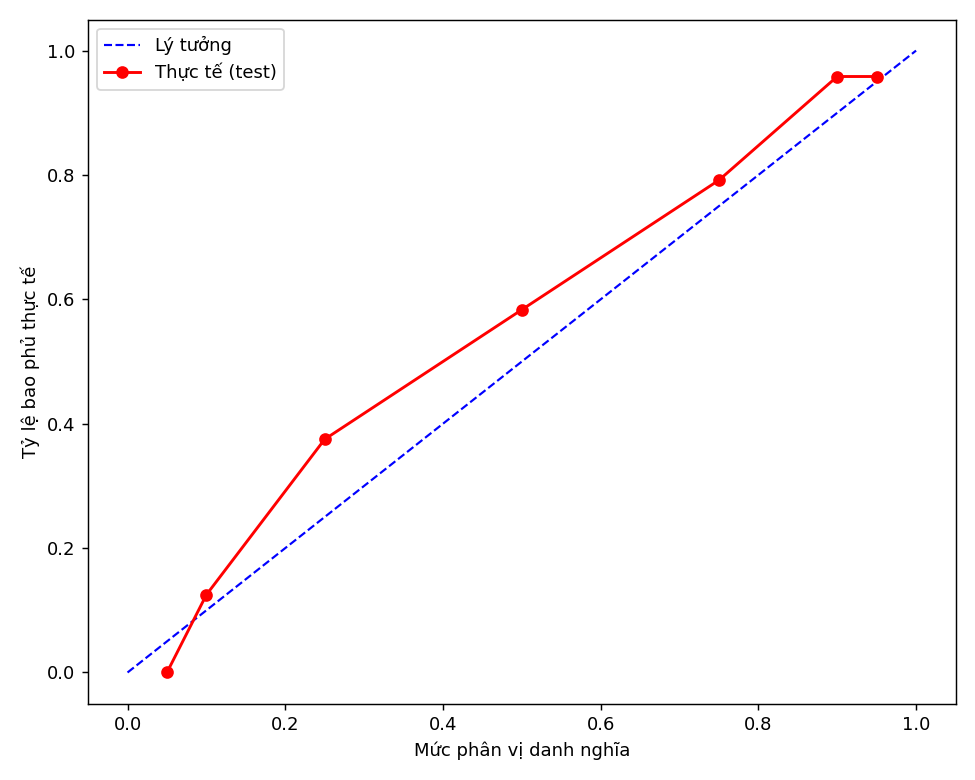
\includegraphics[width=\linewidth]{res3_calibration}
    \end{column}
  \end{columns}
\end{frame}

% ============================================================
\section{Từ dự báo đến quyết định}
% ============================================================

\begin{frame}{Mô hình Newsvendor: phân vị tối ưu}
  \begin{columns}[T]
    \begin{column}{0.5\textwidth}
      Mức tồn kho tối ưu chính là \textbf{phân vị tại tỷ lệ tới hạn}:
      \[ Q^* = F^{-1}(\CR), \quad \CR = \frac{\Cu}{\Cu + \Co} \]
      \vspace{-0.2cm}
      \begin{itemize}\small
        \item Lãi cao ($\Cu$ lớn) $\Rightarrow \CR\!\to\!1 \Rightarrow$ chuẩn bị P90+.
        \item Dễ ế ($\Co$ lớn) $\Rightarrow \CR\!\to\!0 \Rightarrow$ chuẩn bị thấp.
      \end{itemize}
      \vspace{0.15cm}
      {\footnotesize \textbf{Ví dụ 01/2025:} $\Cu{=}30k$, $\Co{=}4k \Rightarrow \CR{=}0{,}88$
      $\Rightarrow$ P88 $\approx 328.300$ $\Rightarrow$ đặt thêm \textbf{228.300}.}
    \end{column}
    \begin{column}{0.5\textwidth}
      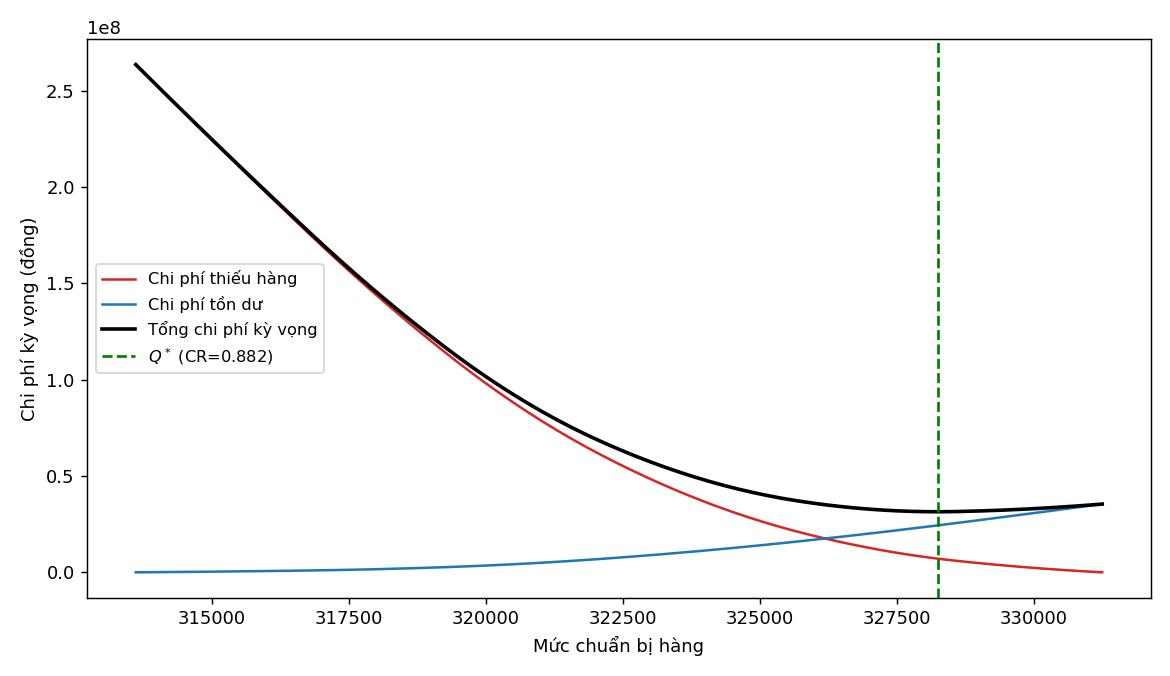
\includegraphics[width=\linewidth]{res4_cost_curve}
    \end{column}
  \end{columns}
\end{frame}

\begin{frame}{Quyết định thay đổi theo cấu trúc chi phí}
  \centering
  \begin{tabular}{rrccr}
    \toprule
    $\Cu$ (đ) & $\Co$ (đ) & \CR & Phân vị & Mức chuẩn bị \\
    \midrule
    30.000 & 10.000 & 0,75 & P75 & 325.646 \\
    30.000 & 4.000  & 0,88 & P88 & 328.254 \\
    30.000 & 1.000  & 0,97 & P97 & 331.250 \\
    10.000 & 30.000 & 0,25 & P25 & 319.299 \\
    \bottomrule
  \end{tabular}
  \vfill
  \begin{exampleblock}{Giá trị của dự báo phân vị}
    Cùng một dự báo nhu cầu, chỉ cần đổi tỉ lệ $\Cu/\Co$, mức chuẩn bị dịch từ
    P25 đến P97 --- điều mà \textbf{dự báo điểm không thể} cung cấp.
  \end{exampleblock}
\end{frame}

\begin{frame}{Triển khai: hai ứng dụng web}
  \begin{columns}[T]
    \begin{column}{0.5\textwidth}
      \begin{block}{Bản kỹ thuật}
        \begin{itemize}\small
          \item Fan chart phân vị P5--P95.
          \item Bảng chỉ số \& calibration.
          \item Newsvendor + EOQ tương tác.
        \end{itemize}
      \end{block}
    \end{column}
    \begin{column}{0.5\textwidth}
      \begin{block}{Bản kinh doanh}
        \begin{itemize}\small
          \item Luồng 3 bước, ngôn ngữ đời thường.
          \item ``Tháng này bán bao nhiêu?'' $\rightarrow$ nhập lãi/lỗ $\rightarrow$ khuyến nghị.
          \item Giải thích bằng lời, không thuật ngữ.
        \end{itemize}
      \end{block}
    \end{column}
  \end{columns}
  \vfill
  \centering\footnotesize Cùng một nền tảng dự báo, phục vụ hai nhóm người dùng khác nhau.
\end{frame}

% ============================================================
\section{Kết luận}
% ============================================================

\begin{frame}{Hạn chế \& hướng phát triển}
  \begin{columns}[T]
    \begin{column}{0.5\textwidth}
      \textbf{Hạn chế}
      \begin{itemize}\small
        \item Tập test còn nhỏ (24 điểm).
        \item Dự báo đệ quy tích lũy sai số.
        \item Mô hình triển khai đơn biến (đa biến để dành mở rộng).
      \end{itemize}
    \end{column}
    \begin{column}{0.5\textwidth}
      \textbf{Hướng phát triển}
      \begin{itemize}\small
        \item Backtest rolling-origin để đánh giá robust.
        \item Kiến trúc đa biến (TFT, iTransformer).
        \item Conformal prediction cho calibration.
      \end{itemize}
    \end{column}
  \end{columns}
\end{frame}

\begin{frame}{Kết luận}
  \begin{enumerate}
    \item \textbf{Dự báo đa phân vị} RevIN + N-BEATS tự triển khai, đạt MAPE
          \textbf{1,15\%} --- vượt baseline $\sim$20 lần; tinh chỉnh Optuna công bằng 5 kiến trúc.
    \item \textbf{Kết nối dự báo $\rightarrow$ quyết định} qua Newsvendor: khuyến nghị
          đặt hàng có cơ sở kinh tế, giải thích được.
    \item \textbf{Hai giao diện web} phục vụ cả kỹ thuật viên lẫn quản lý kinh doanh.
  \end{enumerate}
\end{frame}

\begin{frame}[standout]
  Cảm ơn thầy cô \& các bạn!\\[0.3cm]
  \large Hỏi --- Đáp
\end{frame}

\end{document}
